
\chapter{Fundamentação Teórica}
\label{chap:fundam}
Neste capítulo será discutido na seção 2.1, algumas das ferramentas que já se propõe a realizar
a comparação de moléculas, assim como alguns dos algoritmos que podem ser utilizados na 
análise de similaridade molecular que serão apresentados na seção 2.3, sendo que parte desses 
algoritmos já estão adaptados em algumas das ferramentas a serem apresentadas.
Também será exposto na seção 2.2 algumas formas de representação de uma molécula em um 
ambiente computacional, e sua importância para escolha de qual método de comparação de 
moléculas deverá ser utilizado.
\newpage
\section{FERRAMENTAS PARA COMPUTAÇÃO DE SIMILARIDADE MOLECULAR}

Devido a importância das ferramentas computacionais no processo de descobertas de fármacos, há diversos esforços dedicados ao desenvolvimento destas ferramentas, tornando-as cada vez mais eficientes e eficazes. Como resultado desses esforços, já se encontram disponíveis alguns sistemas computacionais que aplicam algoritmos de similaridade, realizam busca em bancos de dados, predição de propriedades físico-químicas e atividades biológicas, entre outras diversas funcionalidades importantes na pesquisa e desenvolvimento de fármacos. Esses softwares diferenciam-se de acordo com o custo de sua licença, funcionalidades implementadas, formatos de moléculas aceitos, representação computacional da molécula, método de computação de similaridade molecular, entre outros aspectos.

Uma das ferramentas populares entre pesquisadores na área de química medicinal é o ZINC. O sistema web ZINC é uma ferramenta livre que fornece para o usuário um banco de dados com mais de 21 milhões de estruturas catalogadas \cite{irwin2005zinc}. Além disso, o sistema armazena diversas informações  sobre cada molécula como : massa molecular, centros quirais, coeficiente de partição água-etanol calculado (cLogP). O ZINC armazena estruturas em formatos 2D, tal como o formato Simplified Molecular Input Line Entry System (SMILES), que são representações lineares utilizando uma sequência de caracteres para representação da estrutura molecular \cite{kumar2012}. Além do formato SMILES, o ZINC também aceita como formatos de entradas, Structure Data Format (SDF) e MOL2. O ZINC implementa rotinas para triagem virtual em sua base de dados utilizando os conceitos de similaridade molecular, permitindo ao pesquisador selecionar o grau de similaridade mínimo desejado, e retornando todas as moléculas em seu catálogo (banco de dados) com grau de similaridade igual ou superior ao selecionado pelo usuário \cite{irwin2005zinc}. 

\begin{figure}[!htb]
	\centering
	\caption[Exemplo de uma figura]{Exemplo de uma figura onde aparece uma imagem sem nenhum significado especial.}
	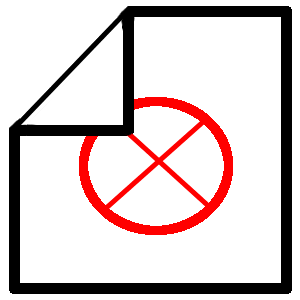
\includegraphics[width=0.2\textwidth]{dummy.png} % <- formatos PNG, JPG e PDF
	\fonte{ABNTEX, 2009\nocite{abnTeX2009}}
	\label{fig:dummy}
\end{figure}